%!TEX root=../../main.tex

\section{Frontend - Webapplikation als REST-Client}
\subsection{Einleitung}
Das \Gls{backend} muss mit dem \Gls{frontend} verbunden werden. Es gibt unterschiedliche Möglichkeiten dies zu realisieren. Beim Realisieren, muss darauf geachtet werden, dass eine Struktur vorhanden ist. Es werden 2 verschiedene \Gls{designpattern} betrachtet und verglichen. Umgesetzt wird dann ein Entwurfsmuster mithilfe von \Gls{js}. Hier kann ein \Gls{js}-\Gls{framework} zum Einsatz kommen. Dazu werden hier verschiedene JavaScript-Frameworks angeschaut und verglichen. Für die Verarbeitung der Daten ist es wichtig Datenformate festzulegen. Die Aufbereitung der Elemente für das Frontend mit den Daten des Backends wird ebenfalls untersucht.
\\\\
Die Fragestellung der Studie ist erstens, welche Unterschiede es bei der Datenrepräsentation und -manipulation zwischen den Entwurfsmustern \Gls{mvvm} und \Gls{mvc} gibt und zweitens, mit welchen Werkzeugen bzw. JavaScript-Frameworks die jeweiligen Methoden zugriffsperformant umgesetzt werden können.
\subsection{Entwurfsmuster}
Dieser Teil des Projektes wird in Verwendung eines Entwurfsmusters umgesetzt. Zwei \Gls{mv*} Entwurfsmuster werden hierbei in Betrachtung gezogen. Zum einen MVVM und zum anderen MVC. Es kommen diese zwei Entwurfsmuster in Frage, da MVC ein sehr bekanntes Entwurfsmuster ist und MVVM eine neuere und spezifischere Variante von MVC ist \cite{mvvm_vue}.
\subsubsection{MVC}
\Gls{mvc} ist ein Entwurfsmuster mit dem eine Software in die drei Teile (Model, View und Controller) geteilt wird \cite{mvc}.\\
Das Model beinhaltet alle Daten der Software und auch alle Funktionen, die mit den Daten interagieren oder mit ihnen rechnen.\\
Die View ist der Teil der Software, den Benutzer sehen und mit denen sie interagieren. Dieser Teil der Software beinhaltet keine wichtigen Daten oder Funktionen, welche Daten bearbeiten. Sie hört nur auf Benutzereingaben und zeigt die bereitgestellten Daten an.\\
Der Controller ist der Teil der Software, der Model und View verbindet. Im Controller wird auf die Benutzereingaben reagiert und werden die gewünschten Funktionen aus dem Model aufgerufen.
\begin{figure}[H]
	\centering
	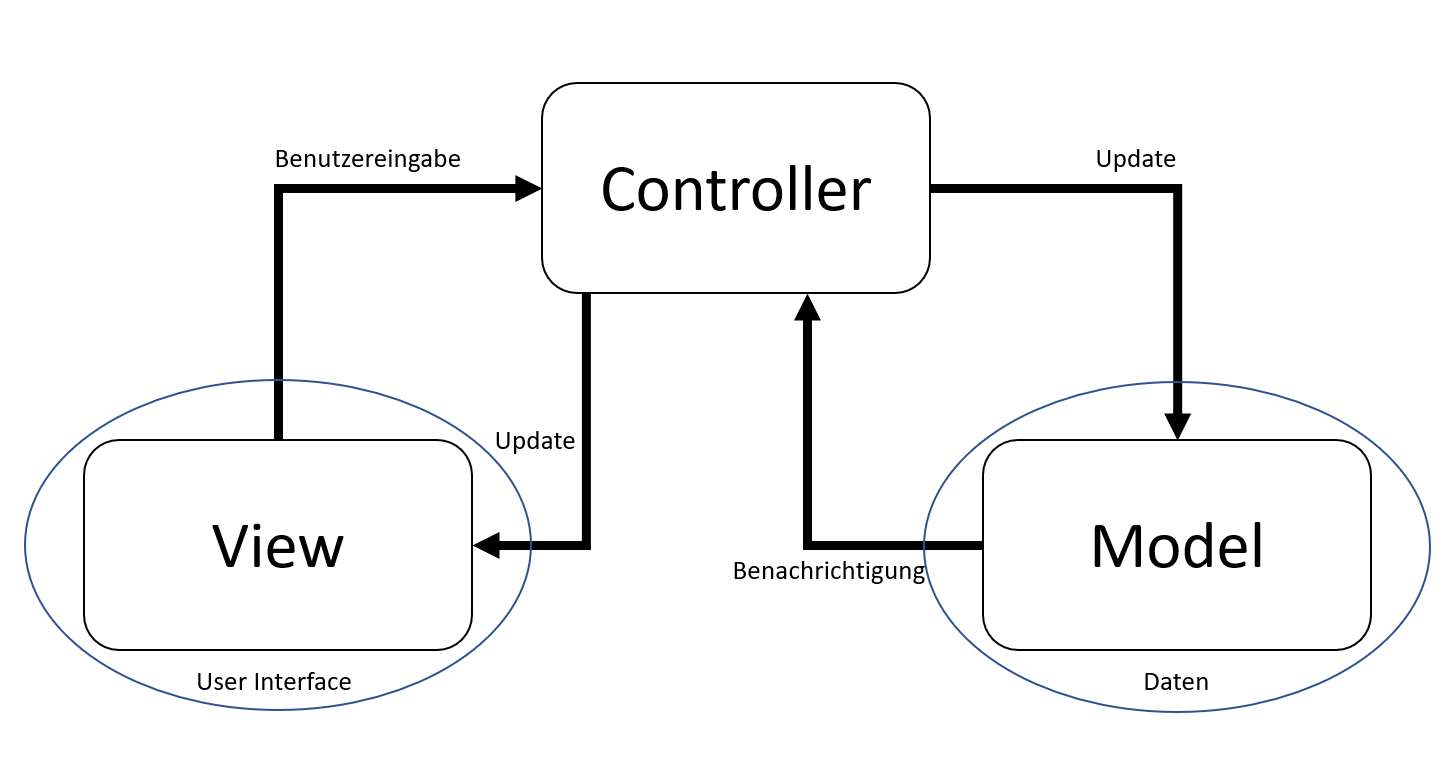
\includegraphics[width=0.8\linewidth]{images/mvc}
	\caption[Übersicht des MVC-Patterns]{Übersicht über die Komponenten des MVC-Patterns und ihre Zusammenhänge}
	\label{fig:mvc}
\end{figure}
\subsubsection{MVVM}
\Gls{mvvm} oder auch \Gls{mvvc} ist ein \Gls{designpattern} mit dem eine Software in drei Teile geteilt wird \cite{mvvm_vue}. Jedoch wird bei MVVM die Software in Model, View und ViewModel aufgeteilt. 
Das Model beinhaltet wie im konventionellen \Gls{mvc}-Pattern alle wichtigen Daten und Funktionen. 
Die View ist wie beim MVC-Pattern der Teil der Software, mit dem der Benutzer interagiert. 
Das ViewModel ist ein Bindeglied zwischen Model und View \cite{mvvm_vue}. Dabei stellt das ViewModel der View Funktionen zur Verfügung. Diese können auch Daten verändern bzw. mit Daten rechnen. Das Model kann über das ViewModel auch mit der View direkt interagieren. 
MVVM sieht nicht vor, dass ein Controller verwendet wird. Diese Funktion übernimmt zu einem gewissen Teil das ViewModel bzw. auch die View und das Model.
\begin{figure}[H]
	\centering
	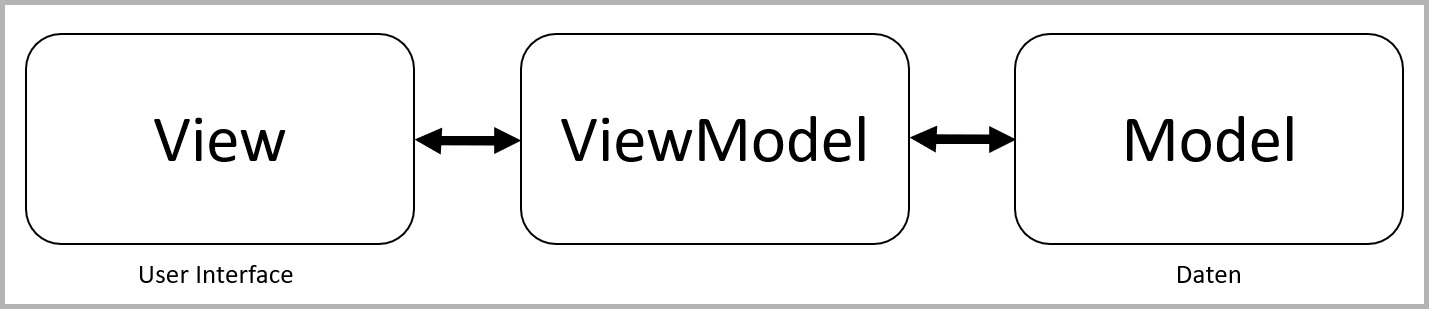
\includegraphics[width=0.8\linewidth]{images/mvvm}
	\caption[Übersicht des MVVM-Patterns]{Übersicht über die Komponenten des MVVM-Patterns und ihre Zusammenhänge}
	\label{fig:mvvm}
\end{figure}
\newpage
\subsubsection{Vergleich}
Diese zwei \Gls{designpattern} sind zwar sehr ähnlich, jedoch gibt es wichtige Unterschiede zwischen ihnen.\\\\
\Gls{mvc} ist ein Entwurfsmuster, welches auf einem niedrigen Level überall im Einsatz ist - z.B. bei Tastatureingaben \cite{mvc}. Dieses Entwurfsmuster ist zwar schon lange verfügbar, jedoch kann es bei Webapplikationen zu Problemen führen.\\
Bei der Entwicklung einer Webapplikation ist es nicht einfach, das Model von dem Controller zu trennen.\\
\Gls{mvvm} auf der anderen Seite zielt explizit auf HTML5 ab \cite{mvvm_vue}. Somit ist es bei webbasierten Applikationen zu bevorzugen.
\subsection{Umsetzungsmöglichkeiten}
Dieser Teil des Projekts wird mittels \Gls{js} umgesetzt. Hierbei kommen unterschiedliche \Gls{js}-\Gls{framework} in Frage. Hier werden die verbreitetsten JavaScript-Frameworks vorgestellt und dann verglichen. \Gls{angular} wird nicht in Betrachtung gezogen, da dies ein \Gls{framework} für professionelle Projekte ist und demnach nicht für vergleichsweise kleine Projekte verwendbar ist, wegen dem Aufwand das Framework zu erlernen \cite{angular_ex}.
\subsubsection{VueJS}
\gls{vue} ist ein progressives JavaScript-Framework. Dies bedeutet, dass VueJS in bereits bestehende Webseiten bzw. in webbasierte Software implementiert werden kann.\\
VueJS kann aber auch von Anfang an verwendet werden, wobei man hier mit den Bibliotheken von VueJS skalieren kann \cite{vuedoc}. VueJS kann Teile einer Webseite in Komponenten aufteilen, um diese mehrmals zu verwenden, falls dies notwendig ist. Jeder dieser Komponenten hat sein eigenes \Gls{html}-, \Gls{css}- und \Gls{js} File, was gebraucht wird, um diese Komponente zu rendern.\\
Um einzelnen Elementen VueJS-Funktionalität zu geben, kann auf diese Elemente folgender Code angewendet werden \cite{vuedoc}:
\begin{code}{html}
	<!DOCTYPE html>
	<html lang="de">
		<head>
			<meta charset="UTF-8">
			<meta name="viewport" content="width=device-width, initial-scale=1.0">
			<title>Kurzes VueJS-Beispiel</title>
		</head>
		<body>
			<h1>Überschrift</h1>
			<div id="app">
				<!-- Der Text, welcher weiter unten Definiert wird, wird hier eingefügt -->
				<!-- Ändert sich die Variable, dann ändert sich auch der Text auf der Webseite -->
				<p> {{ text }} </p>
			</div>
			<script src="https://unpkg.com/vue"></script>
			<script>
				const app = new Vue({
					el: '#app',
					data: {
						text: 'Hier steht Text!'
					}
				})
			</script>
		</body>
	</html>
\end{code}
\captionof{listing}{VueJS Beispiel}
\subsubsection{React}
\Gls{react} ist eine \Gls{js}-Bibliothek, mit der man Benutzeroberflächen entwickeln kann \cite{reactdoc}. React hat wie \Gls{vue} Komponenten. Dies bedeutet, dass man einzelne Elemente mehrfach verwenden kann, falls man dies benötigt.\\
React ist von Facebook entwickelt worden und wurde 2013 als \Gls{opensource}-Lösung veröffentlicht.\\
Folgender Code beschreibt eine Beispiel-React-Webseite \cite{reactdoc}:
\begin{code}{html}
	<!DOCTYPE html>
	<html lang="de">
		<head>
			<meta charset="UTF-8">
			<meta name="viewport" content="width=device-width, initial-scale=1.0">
			<title>Kurzes React-Beispiel</title>
		</head>
		<body>
			<h1>Überschrift</h1>
			<div id="likebuttoncontainer"></div>
			
			<!-- Load React. -->
			<!-- Note: when deploying, replace "development.js" with "production.min.js". -->
			<script src="https://unpkg.com/react@17/umd/react.development.js" crossorigin></script>
			<script src="https://unpkg.com/react-dom@17/umd/react-dom.development.js" crossorigin></script>
			<!-- Load our React component. -->
			<script src="likebutton.js"></script>
		</body>
	</html>
\end{code}
\captionof{listing}{React-Webseite Beispiel}
In der letzten Zeile des body-Tags, wird auf ein "likebutton.js" referenziert. Dies ist eine Komponente und muss noch erstellt werden \cite{reactdoc}:
\begin{code}{js}
	'use strict';
	
	const e = React.createElement;
	
	class LikeButton extends React.Component {
		constructor(props) {
			super(props);
			this.state = { liked: false };
		}
		
		render() {
			if (this.state.liked) {
				return 'You liked this.';
			}
			
			return e(
			'button',
			{ onClick: () => this.setState({ liked: true }) },
			'Like'
			);
		}
	}
	
	const domContainer = document.querySelector('#likebuttoncontainer');
	ReactDOM.render(e(LikeButton), domContainer);
\end{code}
\captionof{listing}{React-Komponente Beispiel}
\subsubsection{Ohne Framework}
Die Schnittstelle zwischen \Gls{backend} und \Gls{frontend} kann auch ohne ein \Gls{framework} umgesetzt werden. Dies ist bei kleinen und leichten Applikationen von Vorteil, da keine umständlichen \Gls{js}-\Gls{framework}s aufgesetzt und richtig implementiert werden müssen. Ohne Framework implementiert man einfach eine \Gls{js}-Datei in eine Webseite, um die gewünschte Funktionalität einzufügen. Mit folgendem Code kann eine Implementierung einer JavaScript-Datei umgesetzt werden:
\begin{code}{html}
	<!DOCTYPE html>
	<html lang="de">
		<head>
			<meta charset="UTF-8">
			<meta name="viewport" content="width=device-width, initial-scale=1.0">
			<title>Kurzes Plain-Beispiel</title>
		</head>
		<body>
			<div id="inhalt">
				<h1>Überschrift</h1>
			</div>
			<!-- Die Implementierung der JavaScript-Datei -->
			<script src="javascript.js"></script>
		</body>
	</html>
\end{code}
\captionof{listing}{Ohne Framework Beispiel}
Es kann auch direkt in ein \Gls{html}-File \Gls{js} in ein <script></script> geschrieben werden.
\subsubsection{Vergleich}
Verglichen werden diese unterschiedlichen Umsetzungsmöglichkeiten an Design, Entwicklungszeit, Performanz und \Gls{loc}.\\
Die Webseite, die für den Vergleich umgesetzt werden soll, wird mit den unterschiedlichen Umsetzungsmöglichkeiten umgesetzt.\\
\begin{figure}[H]
	\centering
	
\includegraphics[width=0.8\linewidth]{images/example_page}
	\caption[Die Beispielwebseite]{Die Beispielwebseite, die mit den Umsetzungsmöglichkeiten umgesetzt werden soll.}
	\label{fig:example}
\end{figure}
Folgende Tabelle zeigt die unterschiedlichen Werte bei der Umsetzung der Beispielwebseite:
\begin{table}
	\captionof{table}{Vergleich von \Gls{js}-\Gls{framework}s}\label{tab:vergleich}
	\centering
	\refstepcounter{table}
	\label{center}
	\begin{tabular}{lcccc}
		Kriterium        & \multicolumn{1}{l}{Maximale Punkte} & \multicolumn{1}{l}{VueJS} & \multicolumn{1}{l}{React} & \multicolumn{1}{l}{Ohne Framework}  \\
		Design           & -                        &            \checkmark               &             \checkmark              &          \checkmark                           \\
		Entwicklungszeit & 10                         &             9              &               7            &               10                      \\
		Performanz       & 10                         &             8              &               5            &                 10                    \\
		\Gls{loc}              & 10                         &             10              &               9            &                   3                  \\
		Gesamtpunkte     & 30                         &              27             &               21            &                23                    
	\end{tabular}
\end{table}
\textbf{Kriterien:}\\\\
\textbf{Design}\\
Das Design fällt in die Wertung, da hier angegeben wird, ob die Beispiel-Website so umgesetzt werden kann, oder ob die Umsetzung in diesem Design nicht möglich ist.\\\\
\textbf{Entwicklungszeit}\\
\Gls{vue}: 40min\\
\Gls{react}: 55min\\
Ohne \Gls{framework}: 20min\\
Die Entwicklungszeit zwischen den zwei \Gls{framework}s ist sehr ähnlich. Jedoch ist zu beachten, dass bei dem VueJS-Framework bereits mit Komponenten gearbeitet worden ist, und dadurch die Entwicklungszeit höher ist als notwendig. Ohne Framework war die Entwicklungszeit am kürzesten, da nichts installiert, importiert oder aufgesetzt werden musste.\\\\
\textbf{Performanz}\\
\Gls{vue}: 112ms\\
\Gls{react}: 175ms\\
Ohne \Gls{framework}: 21ms\\
Ohne Framework ist die Performanz sehr gut, da im Hintergrund keine Frameworks geladen werden müssen. Das \Gls{js} wird direkt ausgeführt. Bei VueJS und React wird viel im Hintergrund geladen und dadurch braucht es länger. Obwohl Komponenten verwendet worden sind, ist VueJS performanter als React.\\\\
\textbf{\Gls{loc}}\\
Die beiden Frameworks haben besonders gut abgeschnitten, da für die Umsetzung mit VueJS nur wenige Codezeilen geschrieben werden mussten sind, da das meiste mit der Funktionalität von VueJS umsetzbar ist. React ist auch sehr gut, da auch sehr wenige Codezeilen geschrieben werden mussten. Jedoch wurde hier allgemein gesagt mehr selbst geschrieben, wodurch es nicht die vollen Punkte erreicht.
Ohne \Gls{framework} gab es am wenigsten Punkte, da die Umsetzung im Vergleich nicht nur unübersichtlich und kompliziert ist, sondern auch damit zu rechnen ist, dass die Umsetzung bei größeren Beispielen noch komplizierter und unübersichtlicher wird.
\subsection{Aufbereitung der Daten}
Die Daten, welche von der REST-Schnittstelle gelesen werden, sind im \Gls{json}-Format. Dies wird genauer im Kapitel \hyperref[sec:json]{Kommunikation und Datenformate} erklärt. Um die Daten von der REST-Schnittstelle zu bekommen, wird \Gls{axios} verwendet. Mit dieser Bibliothek kann eine \Gls{http}-Anfrage gesendet und damit die Daten von der REST-Schnittstelle ausgelesen werden. Im folgenden Code wird eine Beispiel-Anfrage gesendet:
\begin{code}{html}
	<!DOCTYPE html>
	<html>
		<head>
			<!-- Import von Axios -->
			<script src="https://unpkg.com/axios/dist/axios.min.js"></script>
			<meta charset="UTF-8">
			<title>Axios-Anfrage</title>
		</head>
		<body>
			<script>
				// Anfrage an den Server um die Daten zu bekommen
				axios.get("http://localhost:3000/data").then(response => {
					//Die Daten, die zurückkommen werden in der Konsole ausgegeben
					console.log(response.data);
				})
			</script>
		</body>
	</html>
\end{code}
Die Daten, welche von der Anfrage zurückkommen, können dann verwendet werden, um \Gls{html}-Elemente zu erstellen oder zu verändern, um das \Gls{frontend} dynamisch mit den Daten zu füllen.\\Nachdem nicht alle Daten immer gebraucht werden, kann bei den Anfragen die Endung verändert werden, um spezifische Daten abzufragen. Dies muss natürlich von der REST-Schnittstelle unterstützt werden. Eine Beispielanfrage für solch eine spezifische Anfrage ist wie folgt:
\begin{code}{js}
	// Hier werden z.B.: die Daten von dem Benutzer 1234 abgefragt und zurückgegeben.
	axios.get("http://localhost:3000/user/1234/infos").then(response => {
		//Die Daten, die zurückkommen werden in der Konsole ausgegeben
		console.log(response.data);
	})
\end{code}

Die praktische Durchführung ist, wie bereits im vorherigen Kapitel besprochen, bei den Umsetzungsmöglichkeiten unterschiedlich.

\subsection{Fazit}
Nach dieser Arbeit ist die Entscheidung für eine Umsetzungsmöglichkeit relativ leicht. \Gls{mvvm} ist genau auf webbasierte Anwendungen zugeschnitten und bei \Gls{vue} kann durch die vordefinierten Komponenten viel Zeit und Arbeit gespart werden. VueJS hat im Vergleich zu \Gls{react} den Vorteil, das hier bereits mehr Erfahrung in der Umsetzung besteht, woraus folgt, dass VueJS vermutlich die effizienteste Variante für die Umsetzung ist.